\documentclass[a4paper, platex, dvipdfmx]{jsarticle}
\usepackage{graphicx}
\usepackage{amsmath}
\usepackage{float}
\begin{document}
\section{問題}
表1に示す10個の値のペア$(x,y)$の間に、
相関はあるだろうか?

\begin{table}[H]
  \centering
  \caption{今回用いる10個のデータ。}
  \begin{tabular}{ccc}
    \hline
    番号 & $x$の値 & $y$の値 \\\hline
    1 & 51 & 81 \\
    2 & 73 & 15 \\
    3 & 87 & 39 \\
    4 & 4 & 85 \\
    5 & 14 & 84 \\
    6 & 42 & 79 \\
    7 & 22 & 9 \\
    8 & 53 & 30 \\
    9 & 77 & 1 \\
    10 & 79 & 38 \\\hline
  \end{tabular}
\end{table}

\section{散布図を描いてみる}
表1のデータから散布図を描くと、図1のようになる。

\begin{figure}[H]
  \centering
  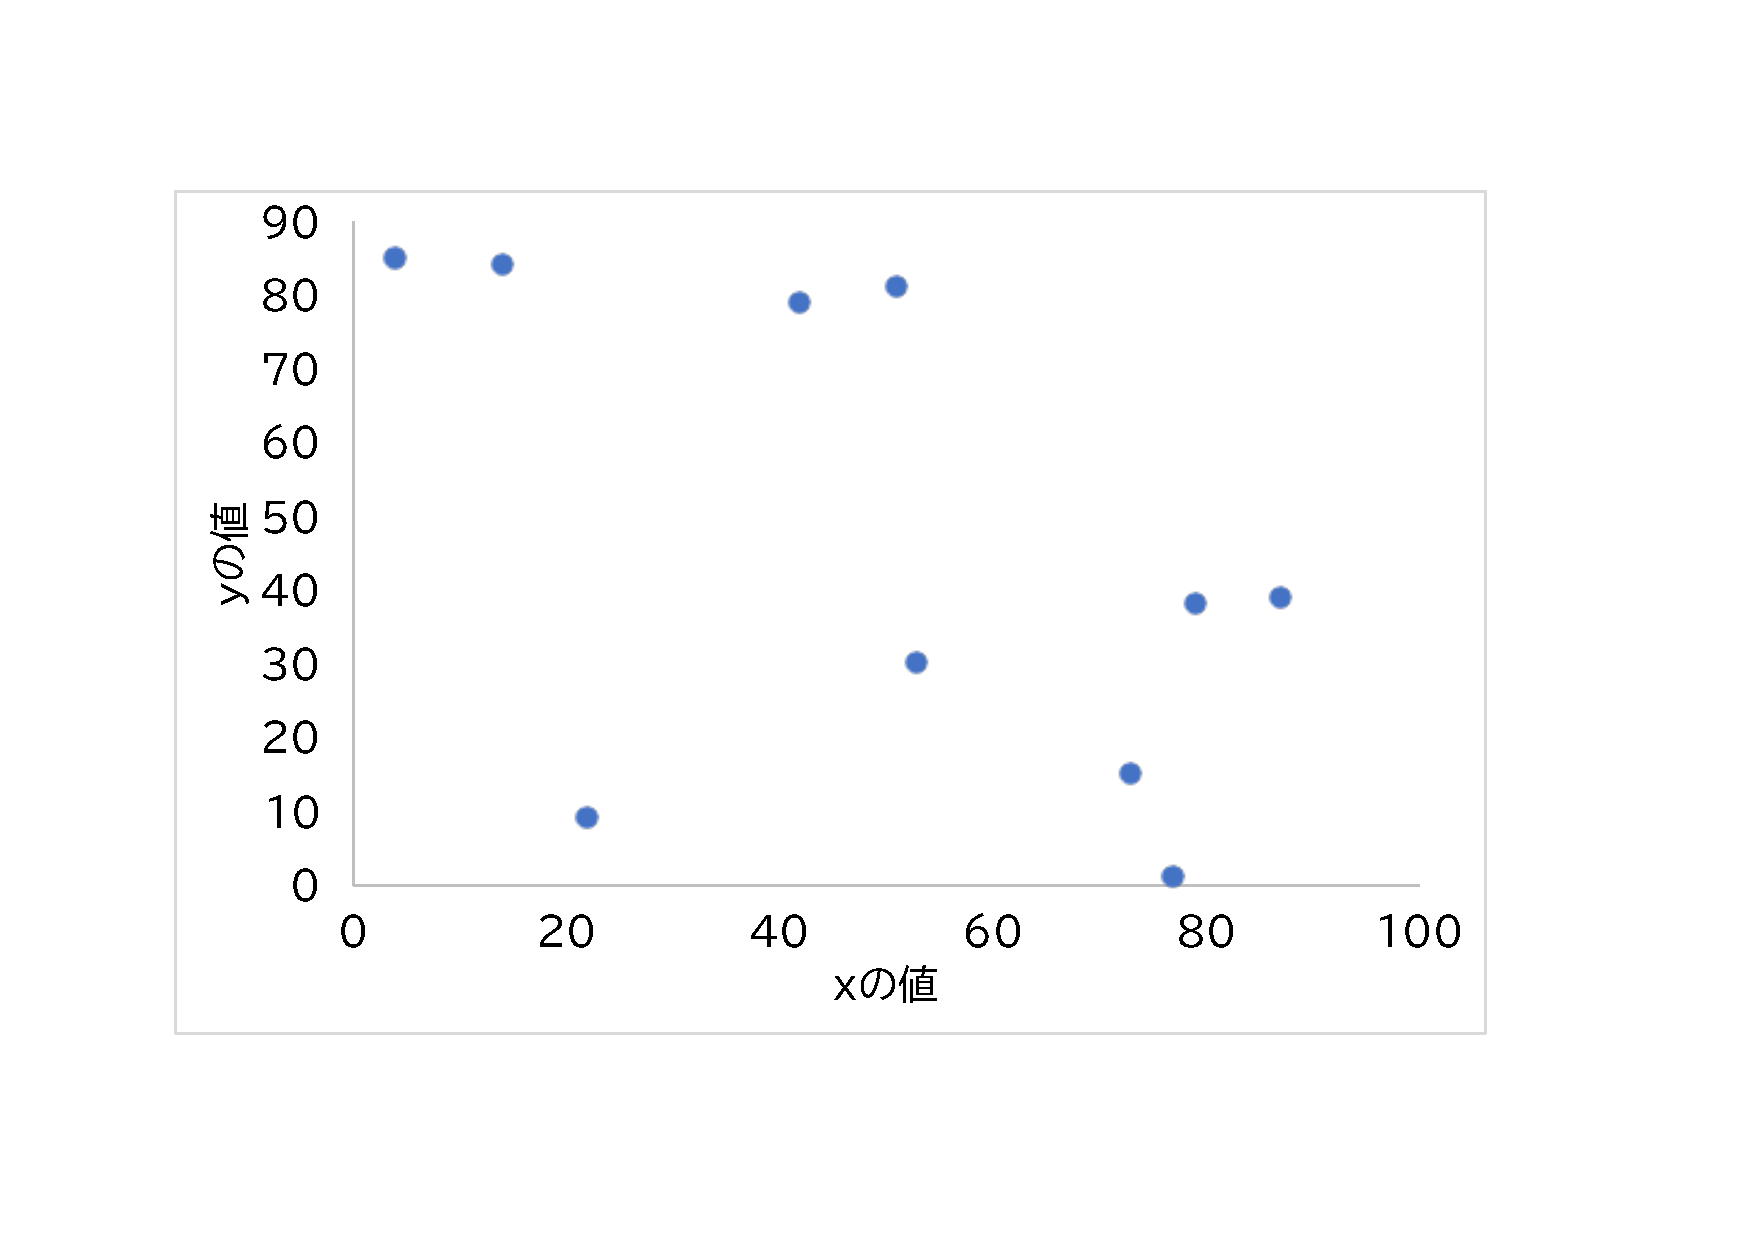
\includegraphics[width=10cm]{cross-ref-scatter.pdf}
  \caption{表1のデータを散布図にしたもの。}
\end{figure}

図1を見る限りでは、相関はなさそうに思える。

\section{相関係数を計算してみる}
第2章では、散布図を描いてみた。
今度は、相関係数を計算してみよう。

10個のデータを$(x_1,y_1),\ldots,(x_{10},y_{10})$と表し、
$x_1,\ldots,x_{10}$の平均値を$\bar{x}$で、
$y_1,\ldots,y_{10}$の平均値を$\bar{y}$で、
それぞれ表すことにする。$x_1,\ldots,x_{10}$と$y_1,\ldots,y_{10}$の間の
相関係数$r$は、次のように定義される。
\begin{align}
  r=\frac{\frac{1}{n}\sum_{k=1}^{10}(x_k-\bar{x})(y_k-\bar{y})}
  {\sqrt{\frac{1}{n}\sum_{k=1}^{10}(x_k-\bar{x})^2}\sqrt{\frac{1}{n}\sum_{k=1}^{10}(y_k-\bar{y})^2}}
\end{align}
式(1)に従って計算すると、$\bar{x}=50.2,\bar{y}=46.1$だから、
\begin{align}
  r=\frac{-4822.2}{7737.6\times 10002.9}=-0.548\cdots
\end{align}
したがって、強い相関があるわけでもないが、全くの無相関でもない程度の
負の相関があることがわかる。
\end{document}